\documentclass[12pt,a4paper]{article}
\renewcommand{\thesection}{\Roman{section}}
\renewcommand{\thesubsection}{\thesection.\Roman{subsection}}
\usepackage{xeCJK}
\usepackage{caption}
\usepackage{amssymb}
\usepackage{amsmath}
\usepackage{geometry}
\usepackage{subfigure}
\usepackage{fancyhdr}
\usepackage[export]{adjustbox}
\usepackage{graphicx}
\graphicspath{{images/}}
\geometry{left=2.5cm,right=1.5cm,top=2cm,bottom=2cm}

\title{Deep Learning and Practice \\Lab2 \\ Report}
\date{April 11, 2019}
\author{呂紹篁, 0751904}
\setCJKmainfont{AR PL UKai CN}
\begin{document}
\captionsetup[figure]{labelfont={bf},labelformat={default},labelsep=period,name={Fig.}}
\thispagestyle{plain}
\cfoot{}
\maketitle

\section{Intoduction} \label{sec:intro}
In this lab, we are aimed to implement simple EEG classification models which are \textbf{EEGNet} and \textbf{DeepConvNet} with \textbf{BCI Competition Dataset}.
Additionally, we need to try three differrent kinds of activation functions, including \textbf{ReLU}, \textbf{Leaky ReLU} and \textbf{ELU}. The trend of training and testing accuracy curves is provided. To compare two models, the tabel of highest testing accuracy of two architecture with three different activation functions is also shown.

\section{Experiment Setup} \label{sec:exp_setup}
\subsection{Detail of Models}
\subsubsection{EEGNet}
Brain computer interfaces (BCI) using neural activity as the control signal to communicate with a computer, the signal is generally chosen from an electroencephalogram (EEG). Lawhern et al. proposed a single CNN archietecture to accurately classify EEG signals from different BCI paradigms \cite{lawhern2018eegnet}. \\
Referred to the archietecture of EEGNet and after several fine-tuned and imporved in our dataset, the network of our EEGNet in PyTorch \cite{paszke2017automatic} is illustrated in Fig. \ref{fig:eegnet}.
\begin{figure}[hbt]
\centering
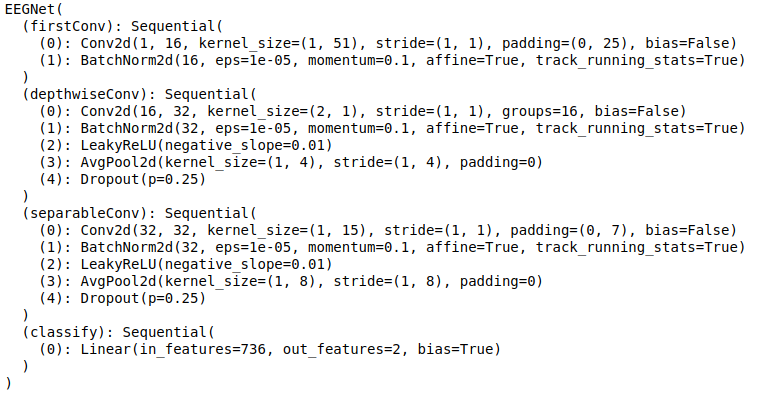
\includegraphics[scale=0.4]{eeg.png}
\caption{Network Architecture of EEGNet}
\label{fig:eegnet}
\end{figure}
\subsubsection{DeepConvNet}
The DeepConvNet was designed to be a \textbf{general-purpose} archietecture that is not restricted to specificx feature types. \cite{lawhern2018eegnet} The network archietecture can be found in the appendix of EEGNet, and after some fine-tuned as well, the result is shown in Fig. \ref{fig:dcn}.
\begin{figure}[hbt]
\centering
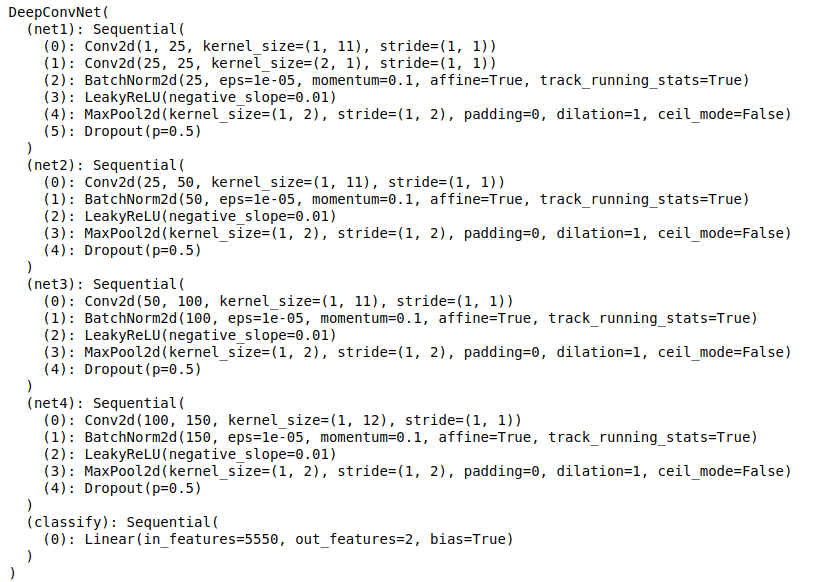
\includegraphics[scale=0.4]{dcn.png}
\caption{Network Architecture of DeepConvNet}
\label{fig:dcn}
\end{figure}

\subsection{Hyper-parameters}
We used whole batch, i.e., batch size equals to \textbf{1080} with \textbf{2000} epochs. For EEGNet, we used constant learning rate which is \textbf{0.005}; for DeepConvNet, the learning rate is time varying which satisfied following equation: 
\begin{align}
\text{learning rate}=
\left\{
  \begin{array}{ll}
  0.005 \text{    if $1 \leq epoch \leq 500$} \\
  0.0025  \text{   if $501 \leq epoch \leq 1000$} \\
  0.00125  \text{  if $1001 \leq epoch \leq 1500$} \\
  0.000625 \text{ if $1501 \leq epoch \leq 2000$} 
  \end{array}
  \right.
\end{align}

\subsection{Activation Functions}
In last lab, we used \textbf{sigmoid} as our activation function. In deep learning, we use \textbf{gradient descent} to optimize the parameters of our model. Thus, gradients, or derivatives, are an important factor effect our result. Observing the derivative of sigmoid, it is clearly that it tends to zero when the magnitude of the input is huge, we called the phenomenon as \textbf{gradient vanishing}, which can caused the neron "dead". ReLU, or rectified linear unit, is a mainstream activation function these days. The concept of ReLU comes from the \textbf{all-or-none principle} of biological neurons: if the stimulus exceeds the threshold potential, the nerve (or muscle fibre) will give a complete response; otherwise, there is no response. 
\begin{itemize}
\item{ReLU} \\
The mathematical representaion of ReLU is pretty simple: $\phi(x) = max(0, x)$. Compare to sigmoid, without exponential computation, ReLU is very easy: we simply compare the input with 0 and output the bigger one. Through it is simple, ReLU is widely used as activation function nowadays. 
\item{Leaky ReLU} \\
While ReLU is very good, there are still some hidden concerns: 1) ReLU is not zero-centered, 2) if unfortunately fall in the interval less than 0, the weights will not be updated, or \textbf{dead ReLU problem}. To solve the issues, there are some derived ReLU family members, for example, \textbf{Leaky ReLU}. Leaky ReLU allow a small, positive gradient when the unit is not active. The mathematical repression of Leaky ReLU is $\phi(x) = max(\alpha x, x)$ where $\alpha$ is a hyper-parameter with small positive value. In PyTorch, $\alpha$ is default to $0.01$.
\item{ELU} \\ 
Exponential linear unit, or ELU, is also a member of ReLU family. ELU try to make the mean activations closer to zero which speeds up learning. ELU can be expressed as 
\begin{align}
\phi(x)=\left\{
                 \begin{array}{ll}
                 x \text{ if $x>0$} \\
                 \alpha (e^x-1) \text{ otherwise}
                 \end{array}
                 \right.
\end{align}
In PyTorch, $\alpha$ is default to $1.0$.
\\
The comparison of three functions is illustrated in Fig. \ref{fig:activation_fun}. For positive parts, three functions are the same. In negative parts, there are only insignificant difference between blue line and green line, however, orange line is totally different.
\begin{figure}[h]
\centering
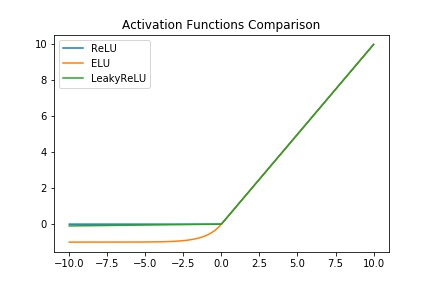
\includegraphics[scale=0.6]{Activation_Functions_Comparison.jpg}
\caption{Comparison of Three Activation Functions}
\label{fig:activation_fun}
\end{figure}

\end{itemize}
\section{Experimental Results} \label{sec:res}
\subsection{Testing Accuracy}
The training and testing accuracy cureves of two models are illustrated in Fig. \ref{fig:acc_com}. From training curves of (a), three activation functions tend to saturated within 500 epochs (from the truth that the training accuracy curves almost equal to 1), and LeakyReLU is fastest one that approaches the border, then ReLU, and the slowest is ELU. Observed the testing curves, ELU remained downtured during all epochs, and the other two are not able to see the superiority. Next, look at the training curves of (b), it is interesting that the order of training speed reversed: ELU, then ReLU, Leaky ReLU be the slowest one this turn. Notice also that the training speed slowed down in general, reached 1 after 750 epochs. Three testing curves are almost closed together and hard to see which one is the best.
\begin{figure}[hbt]
\centering
\subfigure[EEGNet Training and Testing Accuracy Curve]{
  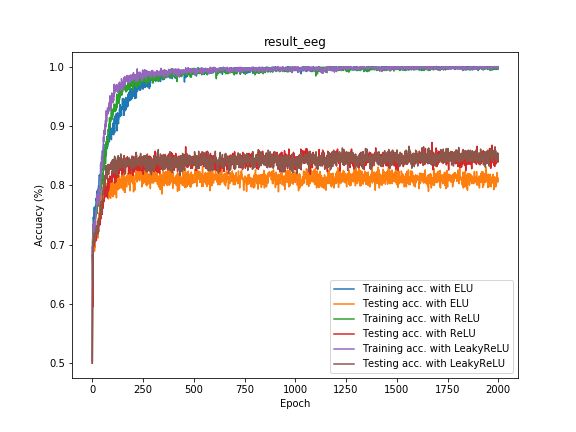
\includegraphics[scale=0.38]{result_eeg.png}
}
\subfigure[DeepConvNet Training and Testing Accuracy Curve]{
  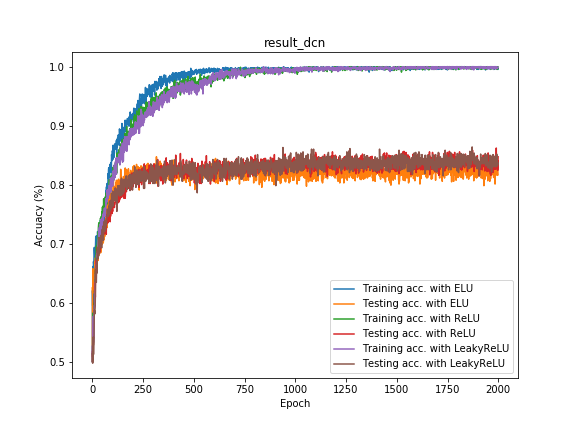
\includegraphics[scale=0.38]{result_dcn.png}
}
\caption{Training and Testing Accuracy Curve Trend}
\label{fig:acc_com}
\end{figure}
\subsection{Comparisons}
The best results of two models testing accuracy are recorded in Tabel \ref{tab:highest} after several trials and attempts. Notice that the results does not correspond to the curves shown in Fig. \ref{fig:acc_com}. It is without surprising that EEGNet performed better then DeepConvNeet. 
\begin{table}[hbt]
\centering
\begin{tabular}{|l|l|l|l|}
\hline
            & ReLU          & Leaky ReLU    & ELU           \\ \hline
EEGNet      & \textbf{87.2} & \textbf{87.6} & 83.6          \\ \hline
DeepConvNet & 86.2          & 86.4          & \textbf{84.8} \\ \hline
\end{tabular}
\caption{Comparison}
\label{tab:highest}
\end{table}
\section{Discussion} \label{sec:dis}
\begin{itemize}
\item{Larger Batch Size Makes Longer Training}
The result is pretty straightforward. Consider batch size 120 and 1080 with 300 epochs. Small batch size will totally update weights $9*300$ times while large batch size will only update $1*300$ times, thus it will spend more time to converge. But as Ian Goodfellow mentioned in \cite{iangoodfellow2016}, for highly curved non-linear cost hyper plane, the approximation (the gradient) will not be very good for very far, so only small step size are safe. 
\item{Revise Kernel Size More Effective Than Channel Size}
During my trial-and-error, I intuitively thought that enlarge the channel sizes can improve the results, but after several trials, this seems not the major factor to effect the result. Then I turned my attention to change the kernel size, though it is annoying to compute the size of each inputs and outputs. The most common problem of changing kernel size is that the size mismatch of fully connected layer, after solving it, every gonna be easy, and I noticed that changing kernel size has more influence than changing channel size. 
\end{itemize}


\bibliographystyle{IEEEtran}
\bibliography{report.bib}

\end{document}
